\documentclass[11pt]{article}
\usepackage{hyperref}
\usepackage[spanish]{babel}
\usepackage[utf8]{inputenc}
\usepackage{pdfpages}
\title{\textbf{Medición de calidad de código en proyectos Open Source en base a métricas}}
\author{Sergio Arroutbi Braojos}
\selectlanguage{spanish}
\date{\today}
\usepackage[bottom=14em]{geometry}
\usepackage{amsmath}
\usepackage{mathtools}
\usepackage{pdflscape}
\usepackage{float}

\begin{document}

\hypersetup
{   
pdfborder={0 0 0}
}
   
\maketitle

\pagebreak

\tableofcontents

\pagebreak

\section{Introducción}

Este documento es una aproximación al mundo de la calidad en el software y, más en concreto, en el código fuente del software libre. La calidad del software es medible, así como también lo es el código fuente que permite construir dicho software. Se define como calidad del software al campo de estudio que describe aquellos atributos de los productos software que son deseables.

Para medir la calidad del código fuente, la utilización de las métricas es fundamental. Se conoce como métrica de software a aquella medida cuantitativa que permite conocer en qué grado un sistema, componente o proceso cumple un atributo determinado ~\cite{ieeeglossary:softwareengineeringterminology}.

Las métricas se han convertido en un ornamento más dentro de las suites de herramientas de gestión del ciclo de vida de desarrollo, proporcionando de un solo vistazo la salud del proyecto a través de paneles de métricas.
El principal problema viene a la hora de conocer qué métricas son más importantes, cuáles lo son menos, cuáles deben tener un seguimiento diario, etc. ~\cite{abistock:usingmetrics}

Dicho lo anterior, cabe destacar que en los proyectos de Software Libre, la propia naturaleza del código fuente, que debe ser accesible de forma pública y usable sin restricciones, hace que la calidad de éste sea aún más importante. El Software Libre es, por su naturaleza, transparencia, y la calidad del código fuente no impacta únicamente en los desarrolladores, sino que es a su vez un factor directamente visible para los potenciales usuarios .
La pretensión de este documento es, en la medida de lo posible, y de forma gradual, intentar llegar a aclarar parte de estos conceptos.

\subsection{Objetivos}
A continuación se definen los objetivos de este documento:
\begin{itemize}
\item{El objetivo de este documento es, en primer lugar, enumerar la existencia de algunos modelos de calidad en el software libre, exponiendo qué carencias muestran a la hora de analizar el código fuente.}
\item{Tras ello, se popondrá un método ligero que permita establecer métricas de análisis de código fuente que permita comparar la calidad de proyectos y justificar qué métricas se definen y en base a qué se evalúan dichas métricas. La principal idea no es llegar a un método eficiente, sino más bien justificar la selección y ponderación de las diversas métricas en base a determinados criterios, de forma que se llegue a la personalización de un modelo de calidad propio para el código fuente}.
\item{Por otro lado, se realizará el estudio, integración e implementación de las herramientas que permitan aglutinar las métricas definidas, así como ponderar cada una de las mismas, para llegar a una evaluación final. Se evaluarán las herramientas existentes en el estado del arte, se realizarán los pasos que permitan integrarlas entre sí y se implmentará un mecanismo que permita su ejecución y sincronización. Se contemplarán, además, aquellas limitaciones existentes, cómo afectan al modelo de calidad establecido y, en qué forma, se podría modificar el modelo para ajustarlo a las herramientas disponibles y al estado del arte de las mismas}.
\item{Finalmente, se realizará un ejemplo práctico de análisis de proyectos de software libre, de forma que se muestre la aplicación del método a través de las herramientas estudiadas para su comparativa. Así, se expondrá la comparativa entre diversos proyectos, de forma que se evalúen dos proyectos de similares características entre sí. Por otro lado, se establecerá el análisis para dos versiones de un mismo proyecto. Esto permitirá conocer el estado del proyecto desde el punto de vista del estado su calidad en función de la progresión del proyecto en el tiempo}.
\end{itemize}

\subsection{Estructura del documento}
Para acometer los objetivos previamente descritos, este documento sigue la siguiente estructura:

\begin{enumerate}
\item{\underline{Introducción}}. Se establecerá una introducción con un resumen de los contenidos del documento. Así se enumerarán en este apartado la misión del documento, los objetivos que éste pretende así como la estructura del documento para enumerar los mismos.
\item{\underline{Modelo de Calidad}}. Como primera aproximación, en este apartado se introducirán los modelos de calidad ya existentes para proyectos de software libre, como OpenBRR, QSOS o QualOSS. Estos modelos, sin embargo, no realizan un análisis avanzado del estado del código y la calidad del mismo, si bien sí que analizan aspectos relacionados con la calidad del código, al menos, indirectamente, como el número de BUGS.
Hilando con esto, se enumerarán distintas métricas que son importantes a la hora de establecer calidad en el software, como por ejemplo desde el número de métodos por clase, número de atributos por clase, dependencias con otras clases, número de parámetros por método o complejidad ciclomática.
Finalmente, en este apartado se debería describir un modelo de calidad basado en métricas software del estilo de OpenBRR pero enfocado única y exclusivamente al análisis de las métricas, con una ponderación que permita establecer la calidad y una justificación de la misma, en cuanto a qué métricas son consideradas más importantes y porqué.
\item{\underline{Herramientas}}. Este apartado permitirá que se describan aquellas herramientas que permiten obtener una o varias de las métricas anteriores, y cómo se pueden combinar dichas herramientas para llegar a la evaluación de calidad final. Se contemplarán, igualmente, herramientas de desarrollo propio o adaptaciones a herramientas ya existentes. Además, se mostrarán diversas gráficas y/o reportes comparativos de la calidad del código para un determinado proyectos.
Así, se podrá mostrar de forma gráfica una comparativa de aquellas métricas más determinantes del sujeto a analizar.
\item{\underline{Caso práctico: MongoDB vs. rethinkdb vs. arangodb}}. En este apartado se realizará el análisis de dos o más proyectos Open Source cualesquiera, de un tamaño similar en líneas de código, escritos en C++. De esta forma, se popdrán concretar los aspectos vistos anteriormente en una comparativa real.
Un ejemplo posible es la comparativa entre bases de datos NoSQL escritas en C++, como pueden ser MongoDB, rethinkdb y arangodb, aunque hay otras opciones. Se puede realizar de igual forma en este apartado más de una comparativa. Se intentará, en todo caso, buscar proyectos escritos en c++, de naturalezas similares, que permitan realizar una comparativa en función de las distintas métricas anteriores.
\item{\underline{Mejoras y posibles trabajos futuros}}. Finalmente, dentro de esta sección, se recogerán mejoras y posibles trabajos futuros que se podrían realizar para mejorar o extender lo que se haya realizado en este proyecto. Se contemplarán, por tanto, opciones de extender el modelo de calidad con más métricas, o bien incluir aspectos que no se han contemplado, extender el modelo para más lenguajes de programación, etc.
\end{enumerate}

\section{Modelo de Calidad}
En esta sección se pretende llegar a un modelo de calidad, basado en métricas, que permita realizar la comparación entre dos o más proyectos de Software Libre, o el estado de uno proyecto a lo largo del tiempo. Así, se estudiará el arte de los modelos de calidad en proyectos de software libre más utilizados en la actualidad, para ver si se pueden reaprovechar en su totalidad, o, al menos, de forma parcial.

Por otro lado, se establecerán diversas métricas que son consideradas en la medición de la calidad de software, tanto desde el punto de vista de programación funcional, como, sobre todo, en el software diseñado en base a orientación a objetos. Además de enumerar las métricas más importantes, se realizará la categorización y priorización de las mismas. Esto permitirá establecer un modelo de calidad en base a métricas según la categorización establecida.

\subsection{Modelos de calidad en proyectos de Software Libre}

Si bien a veces, aunque cada vez menos, los proyectos de Software Libre se consideran caóticos, que su software no es robusto, que no son utilizados por grandes compañías de software o que son, por naturaleza, proyectos que no disponen de soporte, está más que justificado que estas aseveraciones no son más que mitos en torno a este tipo de software ~\cite{oreilly:tenmythsaboutopensourcesoftware}.

El software libre, por estar más expuesto, posee igual o mejor calidad que el software privativo. Además, existen diversos modelos de calidad que permiten establecer la calidad de un proyecto de software libre, y sobre todo comparar la calidad contra otro proyecto de forma que el usuario disponga de información para decantarse en caso de que se tenga que tomar una decisión sobre el software libre que se va a utilizar.

Obviamente, si bien los usuarios finales particulares no someten el software a un modelo de calidad para decantarse por un software libre u otro, y se basan más en una evaluación menos procedimental y más orientada a experiencia de usuario (basada en facilidad de uso, funcionalidad, etc.), sí que es cada vez más común, en el ámbito empresarial, enfrentar varios proyectos de software libre a un modelo de calidad establecido o bien a un modelo de calidad adaptado a las necesidades de la empresa para tomar la decisión de la adquisición final.

Si bien los objetivos de este documento no son realizar un estudio detallado de los modelos de calidad existentes en el Software Libre, sí que resulta interesante presentar dichos modelos para ver qué ofrecen, qué aspectos consideran importantes y qué tipo de evaluación llevan a cabo para establecer sus criterios de calidad.

Antes de hablar de los modelos existentes, cabe destacar que existen dos tipos de modelos de calidad a la hora de evaluar proyectos de Software Libre:

\begin{itemize}
\item{Modelos de calidad ligeros}. Este tipo de modelos son de una implementación más ligera y sencilla respecto a los pesados. Ejemplos de este tipo de modelo son OpenBRR y QSoS.
\item{Modelos de calidad pesados}. Este tipo de modelos, de mayor complejidad y dificultad en su implementación, son considerados más exactos en cuanto a la extensión de su estudio en torno al software.
\end{itemize}

\subsubsection{Modelos Ligeros de Análisis de Calidad del Software Libre}.

Como ya se expuso anteriormente, este tipo de modelos son de sencilla implementación. Así, establecer la calidad de un proyecto de Software Libre puede llegar a ser tan sencillo como rellenar una Hoja de Cálculo con diversas preguntas y ponderar los resultados resultantes. Éste el es caso de OpenBRR.

\begin{itemize}
\item{OpenBRR~\cite{openbrr:openbrr}} (Open Business Readiness Rating). Pese a que en la actualidad se está migrando a un modelo más evolucionado, conocido como OSSpal~\cite{osspal:osspal}, este modelo de calidad ha sido, sin duda, el más sencillo de implementar de los existentes en la actualidad. Como ya se ha comentado, básicamente es una hoja de cálculo que define una serie de super-atributos (conocidos también en el modelo como categorías), con una serie de subcategorías, que no son más que métricas aplicadas a cada una de las categorías. El usuario puede establecer diferentes pesos tanto a la categoría como a las subcategorías. El modelo establece, finalmente, la puntuación final en función de los pesos asignados por el usuario. En la siguiente figura se muestra una de las múltiples categorías del modelo:

\begin{center}
 \begin{figure}[H]
 \begin{center}
   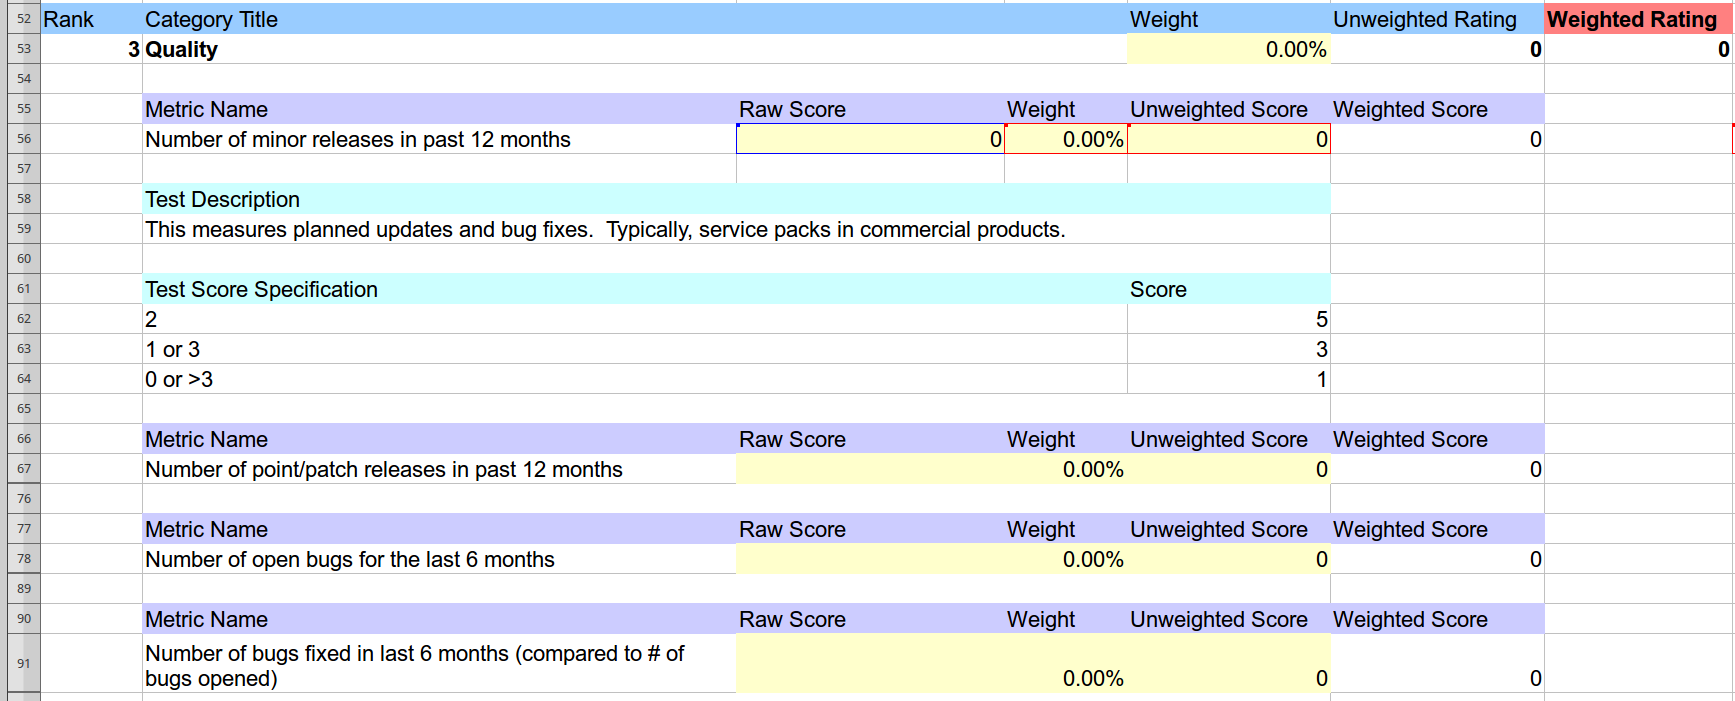
\includegraphics[width=16cm]{img/openbrr_extract00.png}
   \caption{Categoría OpenBRR}
   \label{fig:openbrrcategory}
 \end{center}
 \end{figure}
\end{center}

Las categorías que este modelo propone son las siguientes:
\begin{enumerate}
\item{Funcionalidad}. Grado de cumplimiento de las funcionalidades requeridas.
\item{Usabilidad}. Desde el punto de vista de experiencia de usuario, tiempops de instalación y configuración, etc.
\item{Calidad}. Orientado a número de releases, parches, bugs críticos abiertos o tiempo de resolución de los mismos.
\item{Seguridad}. Número de vulnerabilidades moderadas y/o críticas en determinados períodos de tiempo.
\item{Rendimiento}. Disponibilidad de benchmarks, configuración de performance+tuning, etc.
\item{Escalabilidad}. De forma que se establezca si el software está bien adaptado para ser escalado.
\item{Arquitectura}. Se contemplan, dentro de esta categoría, aspectos como la existencia de plugins de terceros, o si se proporcionan APIs (Application Program Interface)
\item{Soporte}. Se evalúan aspectos como la actividad en las listas de correo del proyecto, o la existencia de soporte profesional y su calidad.
\item{Documentación}. Existencia de documentación variada, desde manuales de usuario, instalación, administración, despliegue o guías de desarrollo.
\item{Adopción}. Esta categoría plantea la existencia de libros en torno al proyecto, o bien la existencia de una base de usuarios real medible.
\item{Comunidad}. Aspectos como el número de contribuidores únicos de código en los últimos meses son los que se contemplan en esta categoría del modelo.
\item{Profesionalismo}. En esta categoría se analizan aspectos como la existencia de un lídel del proyecto o la dificultad que se presenta a la hora de entrar en el equipo de desarrollo.
\end{enumerate}

Como puede observarse en la descripición de la categoría, si bien este modelo no recoge métricas específicas del código fuente, la parte más interesante que presenta es la evaluación de las métricas que realiza, debido, básicamente, a tres aspectos:
\begin{enumerate}
\item{Sencillez}. Este modelo plantea un modo muy sencillo de evaluación de las métricas basado en puntuación más ponderación de cada una de ellas.
\item{Flexibilidad}. La posibilidad de ponderación de cada una de las categorías y subcategorías permite al usuario establecer qué métricas y conjuntos de métricas son las que tienen más impacto a la hora de evaluar la calidad.
\item{Extensibilidad}. El planteamiento que permite este modelo y la fácil implementación de su evaluación permiten extender la evaluación mediante, simplemente, añadir o eliminar categorías o subcategorías según se establezca que es necesario para el usuario final.
\end{enumerate}

Por tanto, si bien OpenBRR no realizar un análisis de métricas de código fuente, su filosofía y la fácil implementación de métricas que el modelo propone pueden servir perfectamente en la evaluación del modelo de calidad del código fuente.

\item{QSOS~\cite{qsos:qsos} (Qualification and Selection of Opensource Software}. Modelo de calidad ligero cuya especificación se establece en el ``QSOS Manifesto''. 
%– QSOS [5]. Qualification and Selection of Opensource Software is a Quality
%Model, licensed under GNU Free Documentation License.
%8The quality model defines what is named as the “QSOS Manifesto”, which
%establishes a list of statements for the objectives that this Quality Model tries
%to define, that can be summarized in:
%∗ Analyzing needs and limitations in software adoption
%∗ Evaluating functional and technical requirements
%∗ Formalizing a methodology
%∗ Results reusing
%∗ Providing a free method
%Based on this manifesto, QSOS defines an iterative process that consist of four
%independent steps:
%∗ Definition. Define a frame of references, with software families, types of
%licenses, types of communities, etc.
%∗ Evaluation. An Evaluation sheet is defined to evaluate the functional
%coverage and the risks that are to be considered from both user and service
%provider perspectives.
%∗ Qualification. This step define filters that take into account needs and
%limitations on the specific context of the project.
%∗ Selection. Identify software meeting the needs and/or requirements. Com-
%pare software and target selection.
%To summarize, this model, despite the fact that is a light-weight model, is,
%somehow, a more difficult model to implement compared to OpenBRR. Apart
%from that, OpenBRR, having the possibility to assign different weights makes
%OpenBRR a more flexible model, more malleable to the necessities and priorities
%of a particular role or a particular company.
%• Heavy-weight: This kind of Quality Models are complex and not easily imple-
%mentable. A good example of this kind of project is QualOSS.
\end{itemize}

\subsubsection{Modelos Pesados de Análisis de Calidad del Software Libre}.
\begin{itemize}
\item{QualOSS}.
%– QualOSS [6]: Quality of Open Source Software. Started on 2006 and funded
%mainly by the European Union, this project aimed to fill the gap in the state of
%the art of the Quality Models for Open Source Project Evaluation.
%It is considered a heavy-weight Quality Model, due to the progress and change
%of methodology that supposed compared to the already existing Quality Models,
%described above.
%One of its first goals consisted of semi-full automation of the analysis of the
%projects and metrics obtaining, by retrieving them using tools such as FLOSS-
%Metrics [7], together with several scripts provided for optimizing this purpose.
%9As this document will not use or even inspire on QualOSS, not very deep infor-
%mation will be provided. However, last but not least, methodology used by this
%Quality Model is exposed below:
%∗ Initial Steps: Consisted of interviews with companies and identification
%of priorities for them when selecting an Open Source Project. One of the
%main priorities identified were the Community, and concepts such as Com-
%munity Side.
%∗ Basic Quality Model: The Methodology followed a GQM (Goal - Ques-
%tion - Metric) basis, where each goal is divided into several questions, and
%several metrics are defined for each question.
%∗ Community Side: The main quality attributes identified for the commu-
%nity side were Size and Regeneration Adequacy, on the one hand, as
%well as Interactivity and Workload Adequacy on the other hand.
%∗ Metrics: The metrics retrieved should be as objective as possible. One of
%more metrics are matched with a given question, and always Metrics were
%result of an average among some data.
\end{itemize}

\subsection{Métricas de diseño orientado a objetos}

\subsubsection{Acoplamiento}
\subsubsection{Cohesión}
\subsubsection{Encapsulación}
\subsubsection{Herencia}
\subsubsection{Complejidad de clases}
\subsubsection{Abstracción}
\subsubsection{Estabilidad}

\subsection{Métricas de calidad de código de clases}
\subsubsection{Número de métodos por clase}
\subsubsection{Número de atributos por clase}

\subsection{Métricas de calidad de código funcional}
\subsubsection{Número de parámetros por método}
\subsubsection{Longitud de métodos}
\subsubsection{Complejidad ciclomática}
\subsubsection{Formateo de código}
\subsubsection{Comentarios de código}

\subsection{Propuesta de modelo de calidad}

\section{Herramientas}

\subsection{Extracción de métricas}

\subsubsection{cccc}

\subsubsection{cppdepend}

\subsubsection{Sonar}

\section{Un ejemplo práctico: MongoDB vs. rethinkdb vs. arangodb}

\subsection{Análisis de la calidad del código}

Esta sección permitirá concretar el modelo de calidad elegido sobre los proyectos inspeccionados. De esta forma, se realizará una comparativa entre los diversos proyectos a analizar.

\subsection{Histórico de calidad del código}

A través de las herramientas descritas anteriormente, se podrá realizar un análisis de la evolución histórica que ha ido sufriendo el código a lo largo del tiempo. De esta forma se podrá identificar si la coumnidad está 

\section{Mejoras y posibles trabajos futuros}

\pagebreak

\bibliographystyle{alpha}
\bibliography{bibliography}
\label{Bibliography}

\end{document}
